% !TEX root = ../vr_st.tex

\subsection{Real projective spaces}\label{s:first_critical_value_rpn}

Let us now focus on the real equatorial system with the antipodal action.
We will consider every sphere \(\bS^n(2)\) to have radius 2 so the quotient \(\rp^n\) has the same diameter as \(\bS^n\).
We will consider reduced (co)homology with mod 2 coefficients.

\medskip\proposition
For \(k,\ell,n,m \in \N\) and \(\Sq^k \in \cO(\ell, k+\ell)\) we have:
\begin{enumerate}
	\item \(\crit(\rp^n) = \frac{2\pi}{3}\).
	\item \(\firstdeath{m}{\rp^n} =
	\begin{cases}
		\frac{\pi}{3} & 1 \leq m \leq n, \\
		\hfil 0 & \text{otherwise}.
	\end{cases}\)
	\item \(\firstdeath{\Sq^k}{\rp^n} =
	\begin{cases}
		\tfrac{\pi}{3} & k \leq \frac{n-1}{2} \text{ and } \binom{\ell}{k} \text{ is odd},\\
		\hfil 0 & \text{otherwise}. \\
	\end{cases}\)
\end{enumerate}

\begin{proof}
	(1) This proposition is stated and proven in \cite[Thm.~4.5]{adams2022metric}.
	
	(2) We only need to prove for the case of $1\leq m\leq n$, since the other case is follows from definition since \(\rH_m(\rp^n) = 0\) if \(m > n\) or \(m = 0\).
	Recall from \cite{katz1983filling} that the filling radius of $\rp^n$ is $\frac{\pi}{3}$ for any $n \geq 1$.
	By \cref{subsub:foundamental_bar_rpn_lemma}, we have that $\firstdeath{m}{\rp^n}\leq \tfrac{\pi}{3}$.
	On the other hand, $\firstdeath{m}{\rp^n}\geq \tfrac{1}{2}\crit(\rp^n) = \tfrac{\pi}{3}$.

	(3) We only need a proof for the case $k \leq \frac{n-1}{2}$ and $\binom{\ell}{k}$ odd, since \(\Sq^k = 0\) otherwise.
	Given that $\VR_r(\rp^n)$ retains the homotopy type of $\rp^n$ for $r \in [0,\tfrac{2\pi}{3})$, \anibal{Recall the cohomology ring in order to use the generator \(\sigma\)} and $\Sq^k(\sigma^\ell) = \binom{\ell}{k}\sigma^{\ell+k}$ generates a bar in $\barc \img_{\Sq^k}$ that is born at $0$ and stays alive until the non-trivial degree-$(\ell+k)$ class $\sigma^{k+\ell}$ dies at $\tfrac{2\pi}{3}$.
	Thus, $\firstdeath{\Sq_\ell^k}{\rp^n} \leq \tfrac{\pi}{3}$.
	On the other hand, $\firstdeath{\Sq^k}{\rp^n} \geq \tfrac{1}{2}\crit(\rp^n) = \tfrac{\pi}{3}$.
\end{proof}

Using the above values, the estimates resulting from the analysis of \cref{ss:barcode_general} are illustrated in \cref{fig:sq barcodes}.

\begin{figure}
	\centering
	\begin{tikzpicture}[scale=0.52]
	\begin{axis} [
		title = {\LARGE $\Hbarc{\degp}{\rp^n},\, \degp\leq n$},
		ticklabel style = {font=\Large},
		axis y line=middle,
		axis x line=middle,
		ytick={0.5,0.67,0.95},
		yticklabels={$\frac{\pi}{2}$,$\frac{2\pi}{3}$,$\pi$},
		xtick={0.5,0.67,0.95},
		xticklabels={$\frac{\pi}{2}$,$\frac{2\pi}{3}$,$\pi$},
		xmin=-0.015, xmax=1.1,
		ymin=0, ymax=1.1,]
		\addplot [mark=none] coordinates {(0,0) (1,1)};
		\addplot [thick,color=black!20!white,fill=black!30!white,
		fill opacity=0.4]coordinates {
			(0.67,0.95)
			(0.67,0.67)
			(0.95,0.95)
			(0.67,0.95)};
		\addplot [black!40!white,mark=none,dashed, thin] coordinates {(0,0.67) (0.67,0.67)};
		%\addplot [black!40!white,mark=none,dashed, thin] coordinates {(0,0.72) (0.72,0.72)};
		\addplot [black!40!white,mark=none,dashed, thin] coordinates {(0.67,0) (0.67,0.67)};
		\addplot[barccolor,mark=*] (0, 0.67) circle (2pt) node[above right,barccolor]{};%{\Large\textsf{1}};
		%\node[mark=none] at (axis cs:0.68,0.21){$\Hbarc{1}{\rp^n}$};
	\end{axis}
\end{tikzpicture}
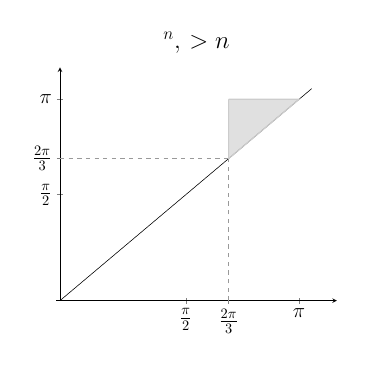
\begin{tikzpicture}[scale=0.52]
	\begin{axis} [
		title={\LARGE $\Hbarc{\degp}{\rp^n},\, \degp>n$},
		ticklabel style = {font=\Large},
		axis y line=middle,
		axis x line=middle,
		ytick={0.5,0.67,0.95},
		yticklabels={$\frac{\pi}{2}$,$\frac{2\pi}{3}$,$\pi$},
		xtick={0.5,0.67,0.95},
		xticklabels={$\frac{\pi}{2}$,$\frac{2\pi}{3}$,$\pi$},
		xmin=-0.015, xmax=1.1,
		ymin=0, ymax=1.1,]
		\addplot [mark=none] coordinates {(0,0) (1,1)};
		\addplot [thick,color=black!20!white,fill=black!30!white,
		fill opacity=0.4]coordinates {
			(0.67,0.95)
			(0.67,0.67)
			(0.95,0.95)
			(0.67,0.95)};
		\addplot [black!40!white,mark=none,dashed, thin] coordinates {(0,0.67) (0.67,0.67)};
		\addplot [black!40!white,mark=none,dashed, thin] coordinates {(0.67,0) (0.67,0.67)};
		% \addplot[barccolor,mark=*] (0, 0.67) circle (2pt) node[above right,barccolor]{\Large\textsf{1}};
		% \node[mark=none] at (axis cs:0.68,0.21){$\Hbarc{\degp}{\rp^n},\, \degp\geq 2$};
	\end{axis}
\end{tikzpicture}

\begin{tikzpicture}[scale=0.52]
	\begin{axis} [
		title = {\LARGE $\sqbarcl{k}{}{\rp^n},\, m \leq n$ and $\binom{m-k}{k}$ odd},
		ticklabel style = {font=\Large},
		axis y line=middle,
		axis x line=middle,
		ytick={0.5,0.67,0.95},
		yticklabels={$\frac{\pi}{2}$,$\frac{2\pi}{3}$,$\pi$},
		xtick={0.5,0.67,0.95},
		xticklabels={$\frac{\pi}{2}$,$\frac{2\pi}{3}$,$\pi$},
		xmin=-0.015, xmax=1.1,
		ymin=0, ymax=1.1,]
		\addplot [mark=none] coordinates {(0,0) (1,1)};
		\addplot [thick,color=black!20!white,fill=black!30!white,
		fill opacity=0.4]coordinates {
			(0.67,0.95)
			(0.67,0.67)
			(0.95,0.95)
			(0.67,0.95)};
		\addplot [black!40!white,mark=none,dashed, thin] coordinates {(0,0.67) (0.67,0.67)};
		%\addplot [black!40!white,mark=none,dashed, thin] coordinates {(0,0.72) (0.72,0.72)};
		\addplot [black!40!white,mark=none,dashed, thin] coordinates {(0.67,0) (0.67,0.67)};
		\addplot[barccolor,mark=*] (0, 0.67) circle (2pt) node[above right,barccolor]{};
        %{\Large$\geq$\textsf{1}};
	\end{axis}
\end{tikzpicture}
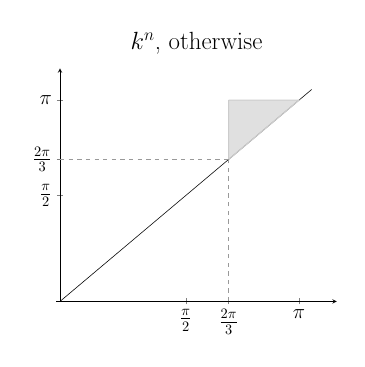
\begin{tikzpicture}[scale=0.52]
	\begin{axis} [
		title={\LARGE $\sqbarcl{k}{}{\rp^n}$, otherwise},
		ticklabel style = {font=\Large},
		axis y line=middle,
		axis x line=middle,
		ytick={0.5,0.67,0.95},
		yticklabels={$\frac{\pi}{2}$,$\frac{2\pi}{3}$,$\pi$},
		xtick={0.5,0.67,0.95},
		xticklabels={$\frac{\pi}{2}$,$\frac{2\pi}{3}$,$\pi$},
		xmin=-0.015, xmax=1.1,
		ymin=0, ymax=1.1,]
		\addplot [mark=none] coordinates {(0,0) (1,1)};
		\addplot [thick,color=black!20!white,fill=black!30!white,
		fill opacity=0.4]coordinates {
			(0.67,0.95)
			(0.67,0.67)
			(0.95,0.95)
			(0.67,0.95)};
		\addplot [black!40!white,mark=none,dashed, thin] coordinates {(0,0.67) (0.67,0.67)};
		\addplot [black!40!white,mark=none,dashed, thin] coordinates {(0.67,0) (0.67,0.67)};
	\end{axis}
\end{tikzpicture}
	\caption{\emph{Top row:} the persistent reduced homology barcode of $\rp^n$.
		%When $1\leq \degp \leq n$, the barcode consists of one $(0,\frac{2\pi}{3})$ and potentially some bars dominated by $(\frac{2\pi}{3}, \pi)$.
		\emph{Bottom row:} the $\img_{\Sq_\ell^k}$-barcode of $\rp^n$.
		%The leftmost barcode contains at least one $(0,\frac{2\pi}{3})$ and potentially some bars dominated by $(\frac{2\pi}{3}, \pi)$;
        %See \cref{s:first_critical_value_rpn} for details.
        In each figure, the gray region represents where additional bars could exist within the corresponding barcode.
	}
	\label{fig:sq barcodes}
\end{figure}